\documentclass[11pt,preprint]{elsarticle}

\usepackage{lmodern}
%%%% My spacing
\usepackage{setspace}
\setstretch{1.2}
\DeclareMathSizes{12}{14}{10}{10}

% Wrap around which gives all figures included the [H] command, or places it "here". This can be tedious to code in Rmarkdown.
\usepackage{float}
\let\origfigure\figure
\let\endorigfigure\endfigure
\renewenvironment{figure}[1][2] {
    \expandafter\origfigure\expandafter[H]
} {
    \endorigfigure
}

\let\origtable\table
\let\endorigtable\endtable
\renewenvironment{table}[1][2] {
    \expandafter\origtable\expandafter[H]
} {
    \endorigtable
}


\usepackage{ifxetex,ifluatex}
\usepackage{fixltx2e} % provides \textsubscript
\ifnum 0\ifxetex 1\fi\ifluatex 1\fi=0 % if pdftex
  \usepackage[T1]{fontenc}
  \usepackage[utf8]{inputenc}
\else % if luatex or xelatex
  \ifxetex
    \usepackage{mathspec}
    \usepackage{xltxtra,xunicode}
  \else
    \usepackage{fontspec}
  \fi
  \defaultfontfeatures{Mapping=tex-text,Scale=MatchLowercase}
  \newcommand{\euro}{€}
\fi

\usepackage{amssymb, amsmath, amsthm, amsfonts}

\def\bibsection{\section*{References}} %%% Make "References" appear before bibliography


\usepackage[numbers]{natbib}

\usepackage{longtable}
\usepackage[margin=2.3cm,bottom=2cm,top=2.5cm, includefoot]{geometry}
\usepackage{fancyhdr}
\usepackage[bottom, hang, flushmargin]{footmisc}
\usepackage{graphicx}
\numberwithin{equation}{section}
\numberwithin{figure}{section}
\numberwithin{table}{section}
\setlength{\parindent}{0cm}
\setlength{\parskip}{1.3ex plus 0.5ex minus 0.3ex}
\usepackage{textcomp}
\renewcommand{\headrulewidth}{0.2pt}
\renewcommand{\footrulewidth}{0.3pt}

\usepackage{array}
\newcolumntype{x}[1]{>{\centering\arraybackslash\hspace{0pt}}p{#1}}

%%%%  Remove the "preprint submitted to" part. Don't worry about this either, it just looks better without it:
\makeatletter
\def\ps@pprintTitle{%
  \let\@oddhead\@empty
  \let\@evenhead\@empty
  \let\@oddfoot\@empty
  \let\@evenfoot\@oddfoot
}
\makeatother

 \def\tightlist{} % This allows for subbullets!

\usepackage{hyperref}
\hypersetup{breaklinks=true,
            bookmarks=true,
            colorlinks=true,
            citecolor=blue,
            urlcolor=blue,
            linkcolor=blue,
            pdfborder={0 0 0}}


% The following packages allow huxtable to work:
\usepackage{siunitx}
\usepackage{multirow}
\usepackage{hhline}
\usepackage{calc}
\usepackage{tabularx}
\usepackage{booktabs}
\usepackage{caption}


\newenvironment{columns}[1][]{}{}

\newenvironment{column}[1]{\begin{minipage}{#1}\ignorespaces}{%
\end{minipage}
\ifhmode\unskip\fi
\aftergroup\useignorespacesandallpars}

\def\useignorespacesandallpars#1\ignorespaces\fi{%
#1\fi\ignorespacesandallpars}

\makeatletter
\def\ignorespacesandallpars{%
  \@ifnextchar\par
    {\expandafter\ignorespacesandallpars\@gobble}%
    {}%
}
\makeatother


% definitions for citeproc citations
\NewDocumentCommand\citeproctext{}{}
\NewDocumentCommand\citeproc{mm}{%
\href{\#cite.\detokenize{#1}}{#2}\nocite{#1}}

\makeatletter
% allow citations to break across lines
\let\@cite@ofmt\@firstofone
% avoid brackets around text for \cite:
\def\@biblabel#1{}
\def\@cite#1#2{{#1\if@tempswa , #2\fi}}
\makeatother
\newlength{\cslhangindent}
\setlength{\cslhangindent}{1.5em}
\newlength{\csllabelwidth}
\setlength{\csllabelwidth}{3em}
\newenvironment{CSLReferences}[2] % #1 hanging-indent, #2 entry-spacing
{\begin{list}{}{%
	\setlength{\itemindent}{0pt}
	\setlength{\leftmargin}{0pt}
	\setlength{\parsep}{0pt}
	% turn on hanging indent if param 1 is 1
	\ifodd #1
	\setlength{\leftmargin}{\cslhangindent}
	\setlength{\itemindent}{-1\cslhangindent}
	\fi
	% set entry spacing
	\setlength{\itemsep}{#2\baselineskip}}}
{\end{list}}

\usepackage{calc}
\newcommand{\CSLBlock}[1]{\hfill\break\parbox[t]{\linewidth}{\strut\ignorespaces#1\strut}}
\newcommand{\CSLLeftMargin}[1]{\parbox[t]{\csllabelwidth}{\strut#1\strut}}
\newcommand{\CSLRightInline}[1]{\parbox[t]{\linewidth - \csllabelwidth}{\strut#1\strut}}
\newcommand{\CSLIndent}[1]{\hspace{\cslhangindent}#1}


\urlstyle{same}  % don't use monospace font for urls
\setlength{\parindent}{0pt}
\setlength{\parskip}{6pt plus 2pt minus 1pt}
\setlength{\emergencystretch}{3em}  % prevent overfull lines
\setcounter{secnumdepth}{5}

%%% Use protect on footnotes to avoid problems with footnotes in titles
\let\rmarkdownfootnote\footnote%
\def\footnote{\protect\rmarkdownfootnote}
\IfFileExists{upquote.sty}{\usepackage{upquote}}{}

%%% Include extra packages specified by user
\usepackage{colortbl}
\providecommand{\pandocbounded}[1]{#1}
\usepackage{chngcntr}
\counterwithout{figure}{section}
\counterwithout{table}{section}\usepackage{booktabs}
\usepackage{longtable}
\usepackage{array}
\usepackage{multirow}
\usepackage{wrapfig}
\usepackage{float}
\usepackage{colortbl}
\usepackage{pdflscape}
\usepackage{tabu}
\usepackage{threeparttable}
\usepackage{threeparttablex}
\usepackage[normalem]{ulem}
\usepackage{makecell}
\usepackage{xcolor}

%%% Hard setting column skips for reports - this ensures greater consistency and control over the length settings in the document.
%% page layout
%% paragraphs
\setlength{\baselineskip}{12pt plus 0pt minus 0pt}
\setlength{\parskip}{12pt plus 0pt minus 0pt}
\setlength{\parindent}{0pt plus 0pt minus 0pt}
%% floats
\setlength{\floatsep}{12pt plus 0 pt minus 0pt}
\setlength{\textfloatsep}{20pt plus 0pt minus 0pt}
\setlength{\intextsep}{14pt plus 0pt minus 0pt}
\setlength{\dbltextfloatsep}{20pt plus 0pt minus 0pt}
\setlength{\dblfloatsep}{14pt plus 0pt minus 0pt}
%% maths
\setlength{\abovedisplayskip}{12pt plus 0pt minus 0pt}
\setlength{\belowdisplayskip}{12pt plus 0pt minus 0pt}
%% lists
\setlength{\topsep}{10pt plus 0pt minus 0pt}
\setlength{\partopsep}{3pt plus 0pt minus 0pt}
\setlength{\itemsep}{5pt plus 0pt minus 0pt}
\setlength{\labelsep}{8mm plus 0mm minus 0mm}
\setlength{\parsep}{\the\parskip}
\setlength{\listparindent}{\the\parindent}
%% verbatim
\setlength{\fboxsep}{5pt plus 0pt minus 0pt}



\begin{document}



\begin{frontmatter}  %

\title{To Stream Or Not To Stream, That Is The Question}

% Set to FALSE if wanting to remove title (for submission)




\author[Add1]{Diaz Sangeve}
\ead{24991422@sun.ac.za}





\address[Add1]{Stellenbosch University, Stellenbosch, South Africa}

\cortext[cor]{Corresponding author: Diaz Sangeve}

\begin{abstract}
\small{
Netflix is built on volume. Up to 2022 its catalogue holds nearly four
thousand films from more than seventy countries, led by the United
States. Each film tradition has a signature, with India leaning on drama
and romance and running a full half hour longer than an American film,
Japan reaching for action, and the United States and Britain heavy with
documentaries. The ratings tell a cautionary tale for a would-be rival,
since the genres that draw the most viewers, thrillers and action, rate
among the lowest, while documentaries earn the highest scores and the
smallest audiences. Set against HBO, Netflix trades quality for breadth,
its median film scoring a full half point lower across every genre. The
lesson for an investor is that breadth fills a catalogue but curation
earns the ratings.
}
\end{abstract}

\vspace{1cm}





\vspace{0.5cm}

\end{frontmatter}

\setcounter{footnote}{0}


\renewcommand{\contentsname}{Table of Contents}
{\tableofcontents}

%________________________
% Header and Footers
%%%%%%%%%%%%%%%%%%%%%%%%%%%%%%%%%
\pagestyle{fancy}
\chead{}
\rhead{}
\lfoot{}
\rfoot{\footnotesize Page \thepage}
\lhead{}
%\rfoot{\footnotesize Page \thepage } % "e.g. Page 2"
\cfoot{}

%\setlength\headheight{30pt}
%%%%%%%%%%%%%%%%%%%%%%%%%%%%%%%%%
%________________________

\headsep 35pt % So that header does not go over title




\newpage

\section*{What works in streaming, read off
Netflix}\label{what-works-in-streaming-read-off-netflix}
\addcontentsline{toc}{section}{What works in streaming, read off
Netflix}

Netflix is the natural place to learn what a streaming catalogue should
look like, and its own slowing growth makes the question timely. Using
the IMDb-sourced record of titles up to 2022, this brief reads the
platform through the four lenses the team asked for, the countries the
films come from, the genres they belong to, the words their descriptions
use, and how they rate and how long they run. Where it helps, the HBO
catalogue from the earlier question sits alongside as a benchmark. The
catalogue runs to 3,759 films and 2,047 shows drawn from 103 countries,
and Figure \ref{catfig} shows how recent and how movie-heavy it is.

\begin{figure}[H]

{\centering 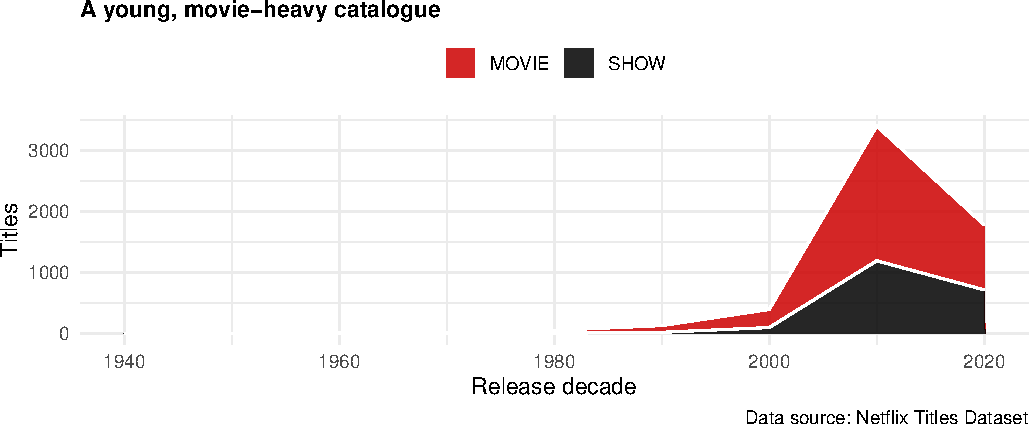
\includegraphics{Question4_files/figure-latex/catfig-1} 

}

\caption{Titles by release decade, films and shows.\label{catfig}}\label{fig:catfig}
\end{figure}

\section*{Where the movies come from}\label{where-the-movies-come-from}
\addcontentsline{toc}{section}{Where the movies come from}

The catalogue is American at its core but far from American alone.
Figure \ref{ctryfig} ranks the production countries, and the United
States leads by a wide margin, with India a clear second ahead of
Britain and France. The presence of India this high is the first sign
that Netflix is not one catalogue but several national ones stacked
together.

\begin{figure}[H]

{\centering 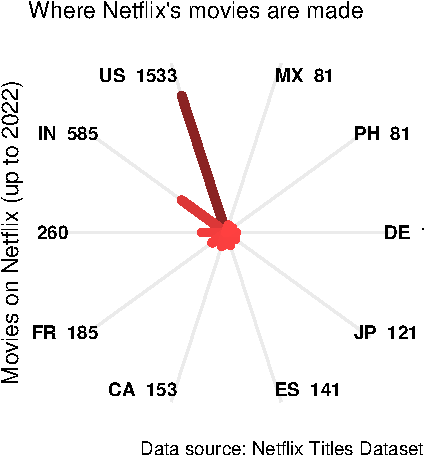
\includegraphics{Question4_files/figure-latex/ctryfig-1} 

}

\caption{Top production countries among films up to 2022.\label{ctryfig}}\label{fig:ctryfig}
\end{figure}

Each of those traditions makes something different. Figure \ref{heatfig}
reads the share of every major producer's films that carry each genre,
and the national signatures are sharp. India leans heavily on drama and
romance, the Bollywood template, while Japan is defined by action far
more than any other country, and the United States and Britain carry the
documentaries. For a rival planning its own slate, the map shows that
genre strategy and sourcing country are the same decision.

\begin{figure}[H]

{\centering 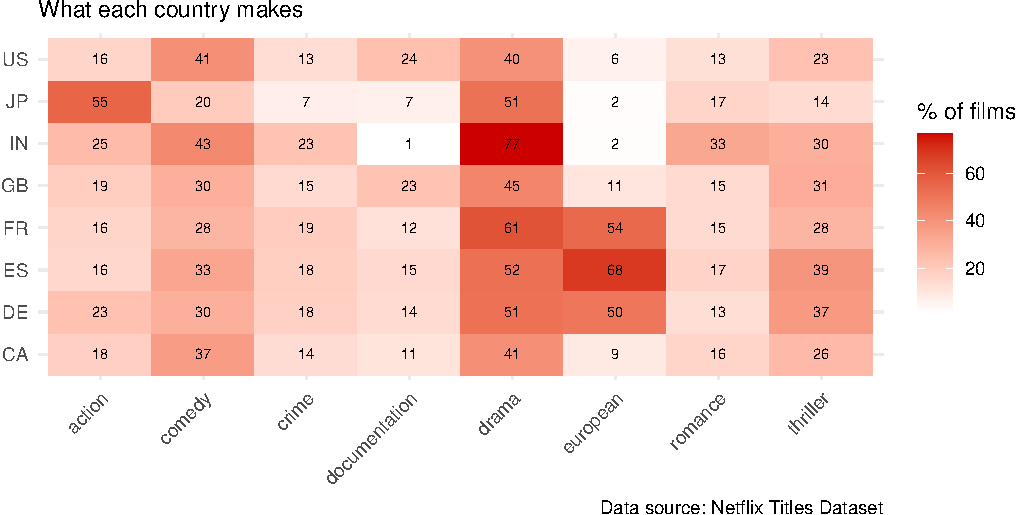
\includegraphics{Question4_files/figure-latex/heatfig-1} 

}

\caption{Share of each country's films carrying each genre. Films can hold more than one genre.\label{heatfig}}\label{fig:heatfig}
\end{figure}

\section*{What the descriptions say}\label{what-the-descriptions-say}
\addcontentsline{toc}{section}{What the descriptions say}

The genres are not just labels, they are written in a distinct language.
Table \ref{wordtab} reports, for each genre, the words most
over-represented in its films' descriptions against the catalogue as a
whole. Thrillers speak of suspects and killers and heists, romances of
crushes and weddings, action of assassins and heroes, and documentaries
of footage and interviews. The text read confirms the genre map and
offers a would-be platform a ready vocabulary for sorting and
recommending its own library.

\begingroup\fontsize{9}{11}\selectfont

\begin{longtable}[t]{ll}
\caption{\label{tab:wordtab}\label{wordtab}Words most distinctive to each genre's descriptions, by lift against the full catalogue}\\
\toprule
Genre & Distinctive words\\
\midrule
action & naruto, assassin, mankind, lord, policeman, hero\\
comedy & hilariously, jokes, laughs, parenting, jeff, riffs\\
crime & serial, heist, criminals, investigation, lord, officers\\
documentation & documentary, unprecedented, interviews, footage, legacy, intimate\\
drama & biopic, aftermath, navigates, tensions, tested, ailing\\
\addlinespace
romance & romantic, handsome, crush, romance, chef, marry\\
thriller & suspects, thriller, investigating, kills, heist, killers\\
\bottomrule
\end{longtable}
\endgroup{}

Genres are not worn one at a time, and how they combine says as much as
how often they appear. Figure \ref{cooccur} reads each cell as the
chance that a film carrying the row genre also carries the column genre,
with the diagonal fixed at one by construction. Drama is the clear hub,
since close to three in four romances and roughly two in three crime and
thriller films are also tagged drama, so a catalogue built on drama
quietly underwrites most of the other genres rather than competing with
them.

\begin{figure}[H]

{\centering 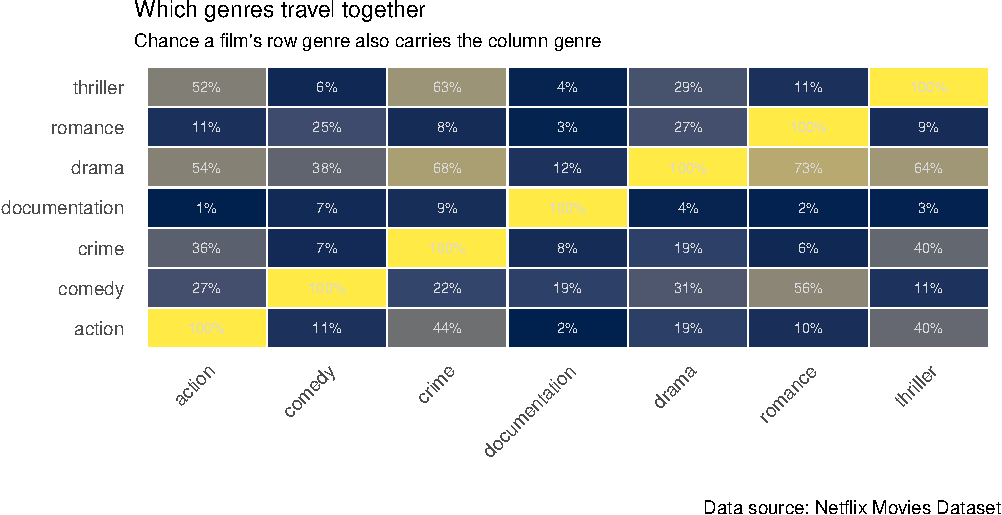
\includegraphics{Question4_files/figure-latex/cooccur-1} 

}

\caption{Conditional genre co-occurrence across films.\label{cooccur}}\label{fig:cooccur}
\end{figure}

\section*{Acclaim and popularity pull
apart}\label{acclaim-and-popularity-pull-apart}
\addcontentsline{toc}{section}{Acclaim and popularity pull apart}

The most useful finding for an investor is that the crowd and the
critics want different things. Figure \ref{ratefig} places each genre by
its median score against its median votes, and the two run in opposite
directions. Thrillers and action draw the largest audiences yet sit near
the bottom for rating, while documentaries earn the highest scores, near
7.1, on the smallest audiences. A thriller pulls a median 9,264 votes
against a documentary's 1,487, so a catalogue chasing both prestige and
reach needs both kinds of title and should not expect one to deliver the
other.

\begin{figure}[H]

{\centering 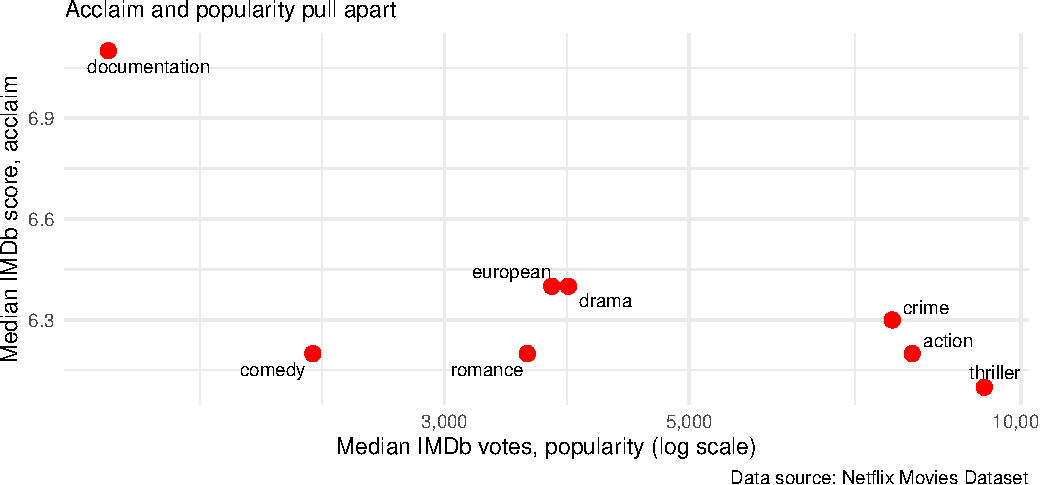
\includegraphics{Question4_files/figure-latex/ratefig-1} 

}

\caption{Median IMDb score against median votes, by genre.\label{ratefig}}\label{fig:ratefig}
\end{figure}

The genre medians hide what individual films do. Figure \ref{scorehex}
bins every film by its score and its audience, with a fitted line
through the cloud. At the film level the tilt is gently positive, with a
correlation near 0.21 between score and log votes, so a more-watched
film tends to rate a little higher even though the genre medians pull
the other way. The contrast is a useful caution, since the divergence
the team should plan around lives at the level of genre strategy, not
within any single title.

\begin{figure}[H]

{\centering 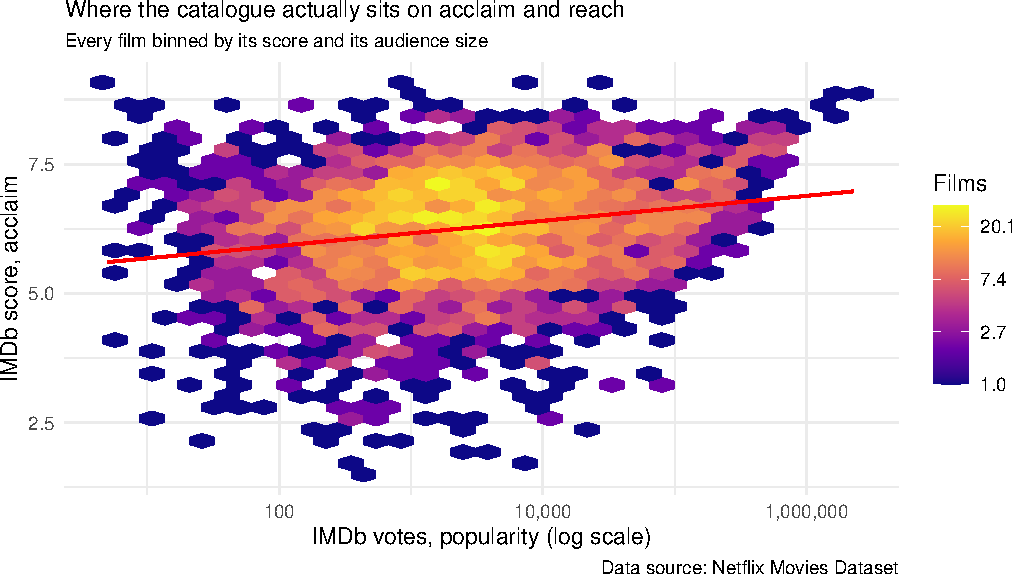
\includegraphics{Question4_files/figure-latex/scorehex-1} 

}

\caption{Film density across IMDb score and votes, with a fitted line.\label{scorehex}}\label{fig:scorehex}
\end{figure}

\section*{How long the movies run}\label{how-long-the-movies-run}
\addcontentsline{toc}{section}{How long the movies run}

Length is another place where the national traditions diverge. Figure
\ref{lenfig} shows the median runtime by country, and India stands apart
at 134 minutes against an American median of 93, a difference of more
than half an hour that reflects the song-and-interval format of
Bollywood cinema. For a platform deciding how to fill a slate, runtime
is not a neutral choice but a fingerprint of where a film was made.

\begin{figure}[H]

{\centering 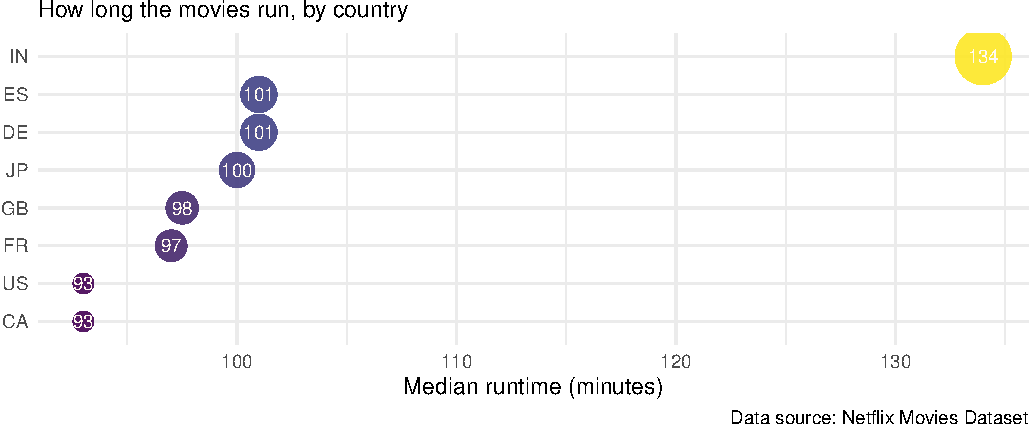
\includegraphics{Question4_files/figure-latex/lenfig-1} 

}

\caption{Median film runtime by country.\label{lenfig}}\label{fig:lenfig}
\end{figure}

The median runtimes earlier hint at a difference that the full
distributions make vivid. Figure \ref{runtimeridges} draws the runtime
distribution for each major producer as a ridge, ordered by the typical
length. The Indian films sit visibly to the right of the American ones
rather than merely averaging higher, so the longer film is the rule
across that tradition and not the work of a few outliers, which is a
real production fact a new entrant would have to budget and schedule
around.

\begin{figure}[H]

{\centering 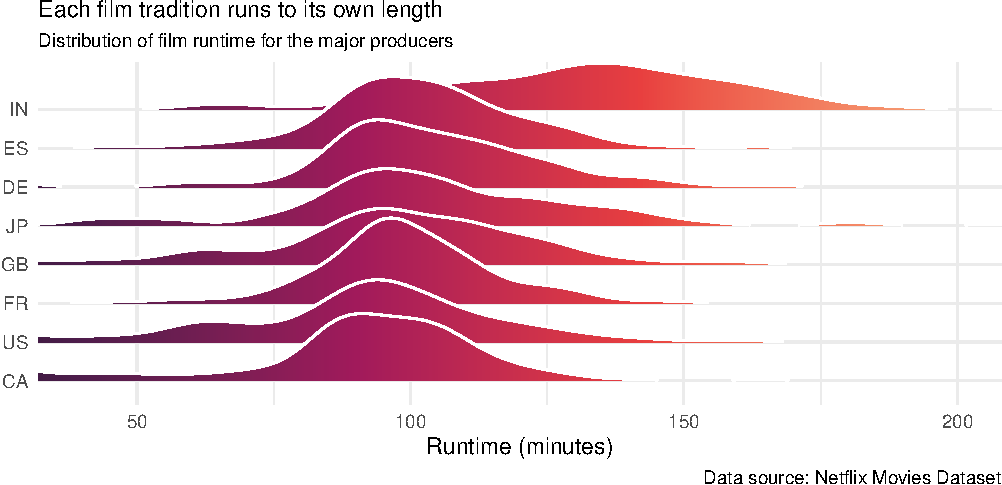
\includegraphics{Question4_files/figure-latex/runtimeridges-1} 

}

\caption{Runtime distribution by major producing country.\label{runtimeridges}}\label{fig:runtimeridges}
\end{figure}

\section*{Netflix set against HBO}\label{netflix-set-against-hbo}
\addcontentsline{toc}{section}{Netflix set against HBO}

A benchmark sharpens the picture, and HBO is the obvious one. Figure
\ref{hbofig} compares the median score of each genre's films across the
two platforms, and HBO sits higher in every single genre. The gap is not
small, with the typical Netflix film scoring 6.4 against HBO's 6.9, a
full half point on the median. Netflix has chosen breadth and HBO has
chosen curation, and the ratings reward the curator. The clearest single
lesson for the team is that a smaller, better-chosen catalogue rates
higher than a larger one.

\begin{figure}[H]

{\centering 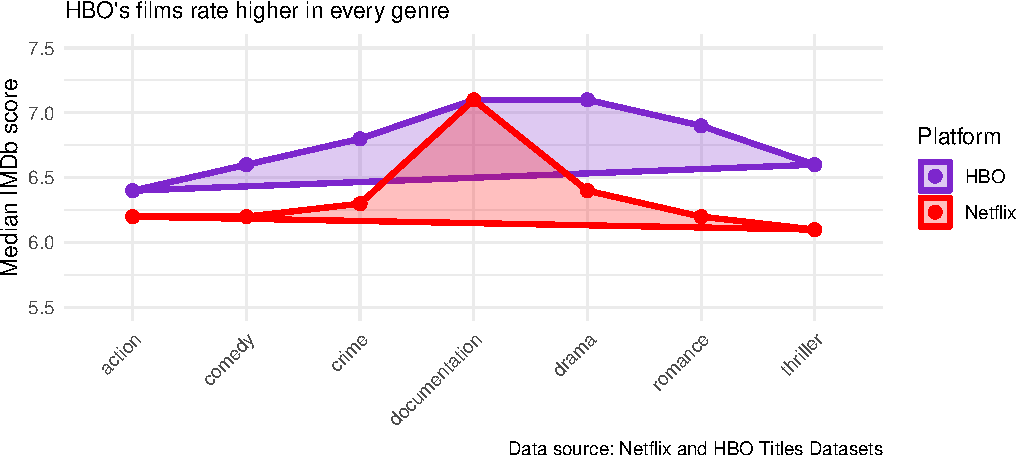
\includegraphics{Question4_files/figure-latex/hbofig-1} 

}

\caption{Median IMDb score per genre, Netflix against HBO films.\label{hbofig}}\label{fig:hbofig}
\end{figure}

\section*{Who and what fills the
shelves}\label{who-and-what-fills-the-shelves}
\addcontentsline{toc}{section}{Who and what fills the shelves}

The people behind the films tell the same story as the map. Table
\ref{actortab} lists the actors credited on the most Netflix films, and
the list is dominated by Bollywood, led by Shah Rukh Khan with 30 films,
which is why India ranks so high. The catalogue also skews mature. Among
the films in the classic export, the single most common age rating is
TV-MA, so adult-oriented content, not family fare, is the platform's
centre of gravity. A new entrant should know that the volume strategy
leans on a few prolific national industries and on mature content to
fill the long tail.

\begin{longtable}[t]{lr}
\caption{\label{tab:actortab}\label{actortab}Actors credited on the most Netflix films up to 2022}\\
\toprule
name & Films\\
\midrule
Shah Rukh Khan & 30\\
Boman Irani & 25\\
Kareena Kapoor Khan & 25\\
Anupam Kher & 24\\
Paresh Rawal & 22\\
\addlinespace
Nawazuddin Siddiqui & 20\\
Priyanka Chopra Jonas & 20\\
Amitabh Bachchan & 19\\
\bottomrule
\end{longtable}

\begin{longtable}[t]{lr}
\caption{\label{tab:agetab}\label{agetab}Most common age ratings among Netflix films (classic catalogue export)}\\
\toprule
Age rating & Films\\
\midrule
TV-MA & 2062\\
TV-14 & 1427\\
R & 797\\
TV-PG & 540\\
PG-13 & 490\\
\addlinespace
PG & 287\\
\bottomrule
\end{longtable}

\section*{The verdict, to stream and
how}\label{the-verdict-to-stream-and-how}
\addcontentsline{toc}{section}{The verdict, to stream and how}

Read through the four lenses the team asked for, Netflix resolves into
one lesson. The platform has chosen volume, holding 3,759 films from 103
countries, and a rival can fill a catalogue the same way, by leaning on
a few productive traditions such as the Indian studio system behind Shah
Rukh Khan and his 30 films. The harder truth sits in the ratings, where
acclaim and reach pull apart, with documentaries scoring highest near
7.1 on the smallest audiences while thrillers draw the largest crowds
and rate among the lowest. No genre delivers both, and the HBO benchmark
drives it home, since HBO outscores Netflix in every genre on the
median, 6.9 against 6.4, a half point bought by curation over scale.

So the answer is to stream, but with intent rather than breadth, a
catalogue built from a few strong production bases, planned genre by
genre, and weighted toward quality where the team most wants to be
judged. That reading carries the limits of its data, since the record
runs only to 2022 and its IMDb scores measure reception rather than
profit, with demand, licensing cost and subscriber behaviour all left
for other evidence to settle. What the catalogue can settle, it does.
Breadth fills the shelves, but curation earns the rating, and a new
entrant should buy the second even at the cost of the first.

\bibliography{Tex/ref}





\end{document}
